\PassOptionsToPackage{unicode=true}{hyperref} % options for packages loaded elsewhere
\PassOptionsToPackage{hyphens}{url}
%
\documentclass[]{article}
\usepackage{lmodern}
\usepackage{amssymb,amsmath}
\usepackage{ifxetex,ifluatex}
\usepackage{fixltx2e} % provides \textsubscript
\ifnum 0\ifxetex 1\fi\ifluatex 1\fi=0 % if pdftex
  \usepackage[T1]{fontenc}
  \usepackage[utf8]{inputenc}
  \usepackage{textcomp} % provides euro and other symbols
\else % if luatex or xelatex
  \usepackage{unicode-math}
  \defaultfontfeatures{Ligatures=TeX,Scale=MatchLowercase}
\fi
% use upquote if available, for straight quotes in verbatim environments
\IfFileExists{upquote.sty}{\usepackage{upquote}}{}
% use microtype if available
\IfFileExists{microtype.sty}{%
\usepackage[]{microtype}
\UseMicrotypeSet[protrusion]{basicmath} % disable protrusion for tt fonts
}{}
\IfFileExists{parskip.sty}{%
\usepackage{parskip}
}{% else
\setlength{\parindent}{0pt}
\setlength{\parskip}{6pt plus 2pt minus 1pt}
}
\usepackage{hyperref}
\hypersetup{
            pdftitle={STAT 542 / CS 598: Project 2},
            pdfauthor={Fall 2019, by Prathamesh(satpute3), Vivek(vivekg3) and Athul(as81)},
            pdfborder={0 0 0},
            breaklinks=true}
\urlstyle{same}  % don't use monospace font for urls
\usepackage[margin=2cm]{geometry}
\usepackage{color}
\usepackage{fancyvrb}
\newcommand{\VerbBar}{|}
\newcommand{\VERB}{\Verb[commandchars=\\\{\}]}
\DefineVerbatimEnvironment{Highlighting}{Verbatim}{commandchars=\\\{\}}
% Add ',fontsize=\small' for more characters per line
\usepackage{framed}
\definecolor{shadecolor}{RGB}{248,248,248}
\newenvironment{Shaded}{\begin{snugshade}}{\end{snugshade}}
\newcommand{\AlertTok}[1]{\textcolor[rgb]{0.94,0.16,0.16}{#1}}
\newcommand{\AnnotationTok}[1]{\textcolor[rgb]{0.56,0.35,0.01}{\textbf{\textit{#1}}}}
\newcommand{\AttributeTok}[1]{\textcolor[rgb]{0.77,0.63,0.00}{#1}}
\newcommand{\BaseNTok}[1]{\textcolor[rgb]{0.00,0.00,0.81}{#1}}
\newcommand{\BuiltInTok}[1]{#1}
\newcommand{\CharTok}[1]{\textcolor[rgb]{0.31,0.60,0.02}{#1}}
\newcommand{\CommentTok}[1]{\textcolor[rgb]{0.56,0.35,0.01}{\textit{#1}}}
\newcommand{\CommentVarTok}[1]{\textcolor[rgb]{0.56,0.35,0.01}{\textbf{\textit{#1}}}}
\newcommand{\ConstantTok}[1]{\textcolor[rgb]{0.00,0.00,0.00}{#1}}
\newcommand{\ControlFlowTok}[1]{\textcolor[rgb]{0.13,0.29,0.53}{\textbf{#1}}}
\newcommand{\DataTypeTok}[1]{\textcolor[rgb]{0.13,0.29,0.53}{#1}}
\newcommand{\DecValTok}[1]{\textcolor[rgb]{0.00,0.00,0.81}{#1}}
\newcommand{\DocumentationTok}[1]{\textcolor[rgb]{0.56,0.35,0.01}{\textbf{\textit{#1}}}}
\newcommand{\ErrorTok}[1]{\textcolor[rgb]{0.64,0.00,0.00}{\textbf{#1}}}
\newcommand{\ExtensionTok}[1]{#1}
\newcommand{\FloatTok}[1]{\textcolor[rgb]{0.00,0.00,0.81}{#1}}
\newcommand{\FunctionTok}[1]{\textcolor[rgb]{0.00,0.00,0.00}{#1}}
\newcommand{\ImportTok}[1]{#1}
\newcommand{\InformationTok}[1]{\textcolor[rgb]{0.56,0.35,0.01}{\textbf{\textit{#1}}}}
\newcommand{\KeywordTok}[1]{\textcolor[rgb]{0.13,0.29,0.53}{\textbf{#1}}}
\newcommand{\NormalTok}[1]{#1}
\newcommand{\OperatorTok}[1]{\textcolor[rgb]{0.81,0.36,0.00}{\textbf{#1}}}
\newcommand{\OtherTok}[1]{\textcolor[rgb]{0.56,0.35,0.01}{#1}}
\newcommand{\PreprocessorTok}[1]{\textcolor[rgb]{0.56,0.35,0.01}{\textit{#1}}}
\newcommand{\RegionMarkerTok}[1]{#1}
\newcommand{\SpecialCharTok}[1]{\textcolor[rgb]{0.00,0.00,0.00}{#1}}
\newcommand{\SpecialStringTok}[1]{\textcolor[rgb]{0.31,0.60,0.02}{#1}}
\newcommand{\StringTok}[1]{\textcolor[rgb]{0.31,0.60,0.02}{#1}}
\newcommand{\VariableTok}[1]{\textcolor[rgb]{0.00,0.00,0.00}{#1}}
\newcommand{\VerbatimStringTok}[1]{\textcolor[rgb]{0.31,0.60,0.02}{#1}}
\newcommand{\WarningTok}[1]{\textcolor[rgb]{0.56,0.35,0.01}{\textbf{\textit{#1}}}}
\usepackage{graphicx,grffile}
\makeatletter
\def\maxwidth{\ifdim\Gin@nat@width>\linewidth\linewidth\else\Gin@nat@width\fi}
\def\maxheight{\ifdim\Gin@nat@height>\textheight\textheight\else\Gin@nat@height\fi}
\makeatother
% Scale images if necessary, so that they will not overflow the page
% margins by default, and it is still possible to overwrite the defaults
% using explicit options in \includegraphics[width, height, ...]{}
\setkeys{Gin}{width=\maxwidth,height=\maxheight,keepaspectratio}
\setlength{\emergencystretch}{3em}  % prevent overfull lines
\providecommand{\tightlist}{%
  \setlength{\itemsep}{0pt}\setlength{\parskip}{0pt}}
\setcounter{secnumdepth}{0}
% Redefines (sub)paragraphs to behave more like sections
\ifx\paragraph\undefined\else
\let\oldparagraph\paragraph
\renewcommand{\paragraph}[1]{\oldparagraph{#1}\mbox{}}
\fi
\ifx\subparagraph\undefined\else
\let\oldsubparagraph\subparagraph
\renewcommand{\subparagraph}[1]{\oldsubparagraph{#1}\mbox{}}
\fi

% set default figure placement to htbp
\makeatletter
\def\fps@figure{htbp}
\makeatother

\usepackage{etoolbox}
\makeatletter
\providecommand{\subtitle}[1]{% add subtitle to \maketitle
  \apptocmd{\@title}{\par {\large #1 \par}}{}{}
}
\makeatother
\usepackage[ruled,vlined,linesnumbered]{algorithm2e}
% https://github.com/rstudio/rmarkdown/issues/337
\let\rmarkdownfootnote\footnote%
\def\footnote{\protect\rmarkdownfootnote}

% https://github.com/rstudio/rmarkdown/pull/252
\usepackage{titling}
\setlength{\droptitle}{-2em}

\pretitle{\vspace{\droptitle}\centering\huge}
\posttitle{\par}

\preauthor{\centering\large\emph}
\postauthor{\par}

\predate{\centering\large\emph}
\postdate{\par}
\usepackage{booktabs}
\usepackage{longtable}
\usepackage{array}
\usepackage{multirow}
\usepackage{wrapfig}
\usepackage{float}
\usepackage{colortbl}
\usepackage{pdflscape}
\usepackage{tabu}
\usepackage{threeparttable}
\usepackage{threeparttablex}
\usepackage[normalem]{ulem}
\usepackage{makecell}
\usepackage{xcolor}

\title{STAT 542 / CS 598: Project 2}
\author{Fall 2019, by Prathamesh(satpute3), Vivek(vivekg3) and Athul(as81)}
\date{Due: Monday, Dec 16 by 11:59 PM Pacific Time}

\begin{document}
\maketitle

\hypertarget{points-half-a-page-project-description-and-summary.-this-part-should-summerise-your-goal-your-approach-and-your-results.}{%
\subsubsection{{[}10 Points, half a page{]} Project description and
summary. This part should summerise your goal, your approach, and your
results.}\label{points-half-a-page-project-description-and-summary.-this-part-should-summerise-your-goal-your-approach-and-your-results.}}

half page description goes here

\hypertarget{points-half-a-page-data-processing-for-question-1.-describe-how-you-process-the-data-so-that-it-can-be-analyzed-to-answer-question-1.}{%
\subsubsection{{[}5 Points, half a page{]} Data processing for Question
1. Describe how you process the data so that it can be analyzed to
answer question
1.}\label{points-half-a-page-data-processing-for-question-1.-describe-how-you-process-the-data-so-that-it-can-be-analyzed-to-answer-question-1.}}

half page description goes here

\hypertarget{points-within-5-pages-classification-models-based-on-pixels.}{%
\subsubsection{{[}30 Points, within 5 pages{]} Classification models
based on
pixels.}\label{points-within-5-pages-classification-models-based-on-pixels.}}

\begin{Shaded}
\begin{Highlighting}[]
  \CommentTok{# kable(results, caption = "KNN")}
\end{Highlighting}
\end{Shaded}

\begin{Shaded}
\begin{Highlighting}[]
\CommentTok{# use parallel for performace }
  \KeywordTok{registerDoMC}\NormalTok{(}\DataTypeTok{cores =} \DecValTok{4}\NormalTok{)}
\NormalTok{  cv_glmnet_model <-}\StringTok{ }\KeywordTok{cv.glmnet}\NormalTok{(train.data[, }\DecValTok{-1}\NormalTok{], train.data[, }\DecValTok{1}\NormalTok{], }\DataTypeTok{parallel =} \OtherTok{TRUE}\NormalTok{, }\DataTypeTok{alpha=}\DecValTok{1}\NormalTok{, }\DataTypeTok{family=}\StringTok{"binomial"}\NormalTok{)}
\end{Highlighting}
\end{Shaded}

\begin{center}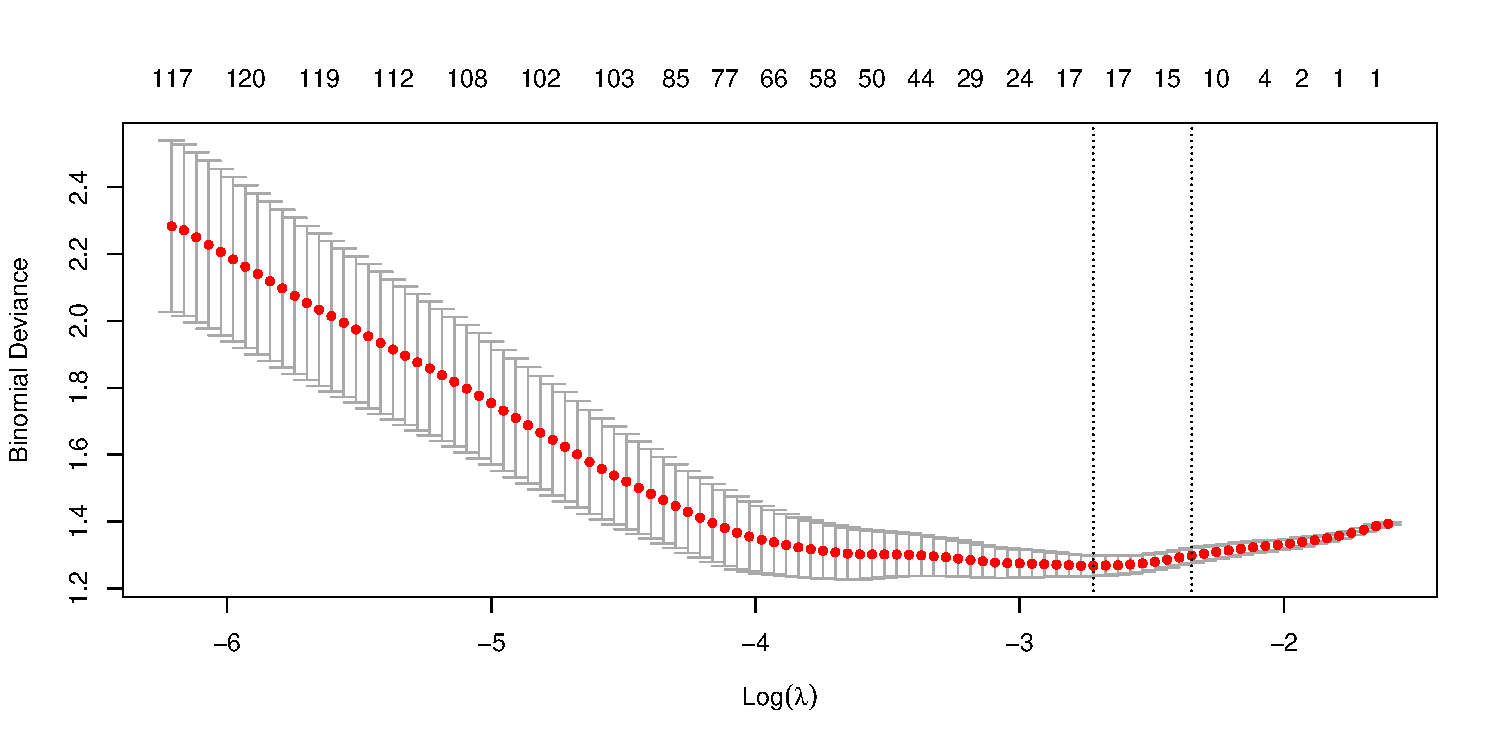
\includegraphics[width=1\linewidth]{Project2_as81_files/figure-latex/unnamed-chunk-11-1} \end{center}

\begin{Shaded}
\begin{Highlighting}[]
\NormalTok{  best_lambda =}\StringTok{ }\NormalTok{cv_glmnet_model}\OperatorTok{$}\NormalTok{lambda}\FloatTok{.1}\NormalTok{se}
  \CommentTok{# training with best lambda selected from the cv}
\NormalTok{  train_glmnet_model <-}\StringTok{ }\KeywordTok{glmnet}\NormalTok{(train.data[, }\DecValTok{-1}\NormalTok{], train.data[, }\DecValTok{1}\NormalTok{], }\DataTypeTok{lambda =}\NormalTok{ best_lambda, }\DataTypeTok{alpha=}\DecValTok{1}\NormalTok{, }\DataTypeTok{family=}\StringTok{"binomial"}\NormalTok{)}
  
  \KeywordTok{summary}\NormalTok{(train_glmnet_model)}
\end{Highlighting}
\end{Shaded}

\begin{verbatim}
##            Length Class     Mode     
## a0             1  -none-    numeric  
## beta       30000  dgCMatrix S4       
## df             1  -none-    numeric  
## dim            2  -none-    numeric  
## lambda         1  -none-    numeric  
## dev.ratio      1  -none-    numeric  
## nulldev        1  -none-    numeric  
## npasses        1  -none-    numeric  
## jerr           1  -none-    numeric  
## offset         1  -none-    logical  
## classnames     2  -none-    character
## call           6  -none-    call     
## nobs           1  -none-    numeric
\end{verbatim}

\begin{Shaded}
\begin{Highlighting}[]
\NormalTok{  pred <-}\StringTok{ }\KeywordTok{predict}\NormalTok{(train_glmnet_model, }\DataTypeTok{s =}\NormalTok{ best_lambda, }\DataTypeTok{newx =}\NormalTok{ test.data[, }\DecValTok{-1}\NormalTok{], }\DataTypeTok{type =} \StringTok{"class"}\NormalTok{)}
\NormalTok{  accuracy =}\StringTok{ }\KeywordTok{mean}\NormalTok{(test.data[, }\DecValTok{1}\NormalTok{] }\OperatorTok{==}\StringTok{ }\NormalTok{pred)}
  
\NormalTok{  results =}\StringTok{ }\KeywordTok{data.frame}\NormalTok{(}\StringTok{"Best lambda"}\NormalTok{ =}\StringTok{ }\NormalTok{best_lambda, }\StringTok{"Accuracy"}\NormalTok{ =}\StringTok{ }\NormalTok{accuracy)}
\end{Highlighting}
\end{Shaded}

\begin{Shaded}
\begin{Highlighting}[]
  \KeywordTok{kable}\NormalTok{(results, }\DataTypeTok{caption =} \StringTok{"Lasso Regression Results"}\NormalTok{)}
\end{Highlighting}
\end{Shaded}

\begin{table}

\caption{\label{tab:unnamed-chunk-13}Lasso Regression Results}
\centering
\begin{tabular}[t]{r|r}
\hline
Best.lambda & Accuracy\\
\hline
0.0954646 & 0.6333333\\
\hline
\end{tabular}
\end{table}

\begin{center}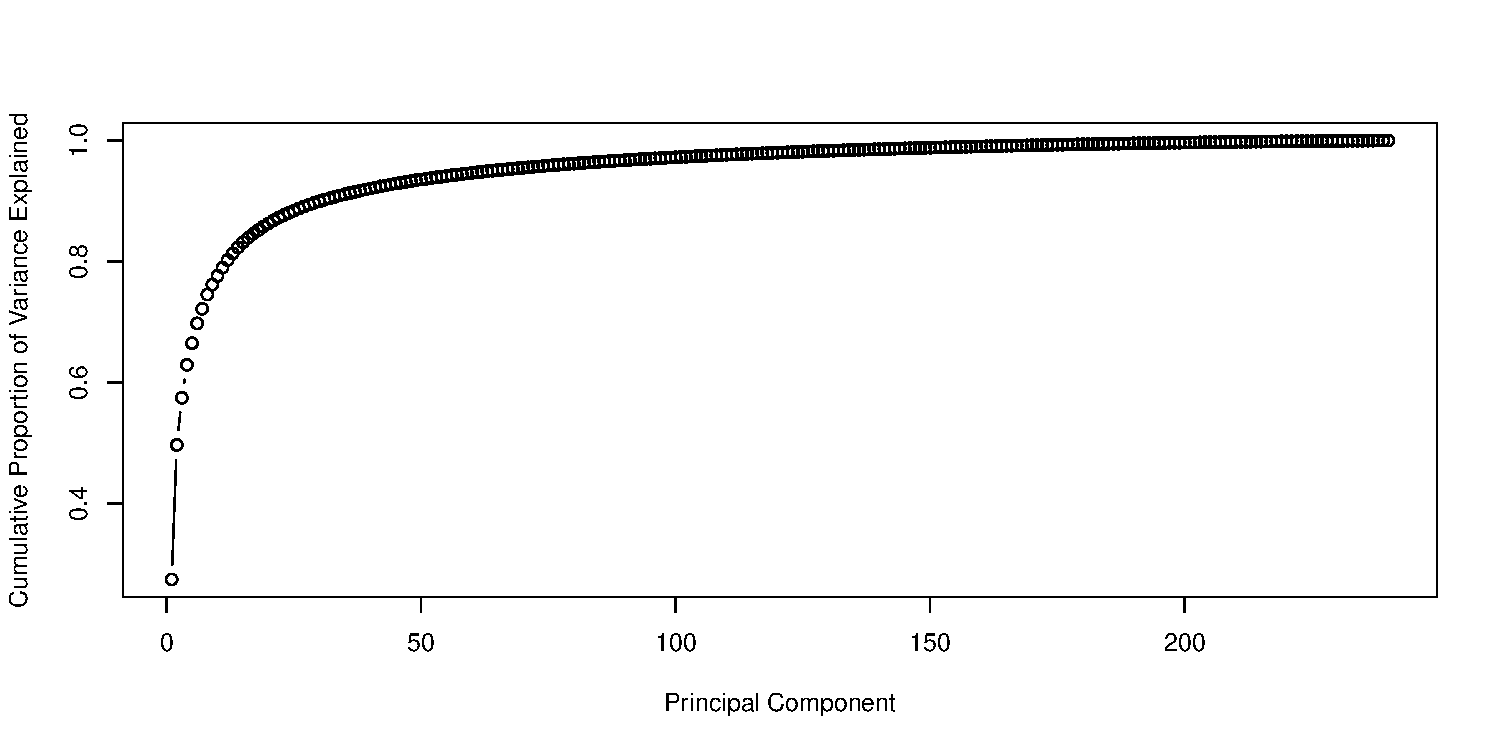
\includegraphics[width=1\linewidth]{Project2_as81_files/figure-latex/unnamed-chunk-16-1} \end{center}

\begin{center}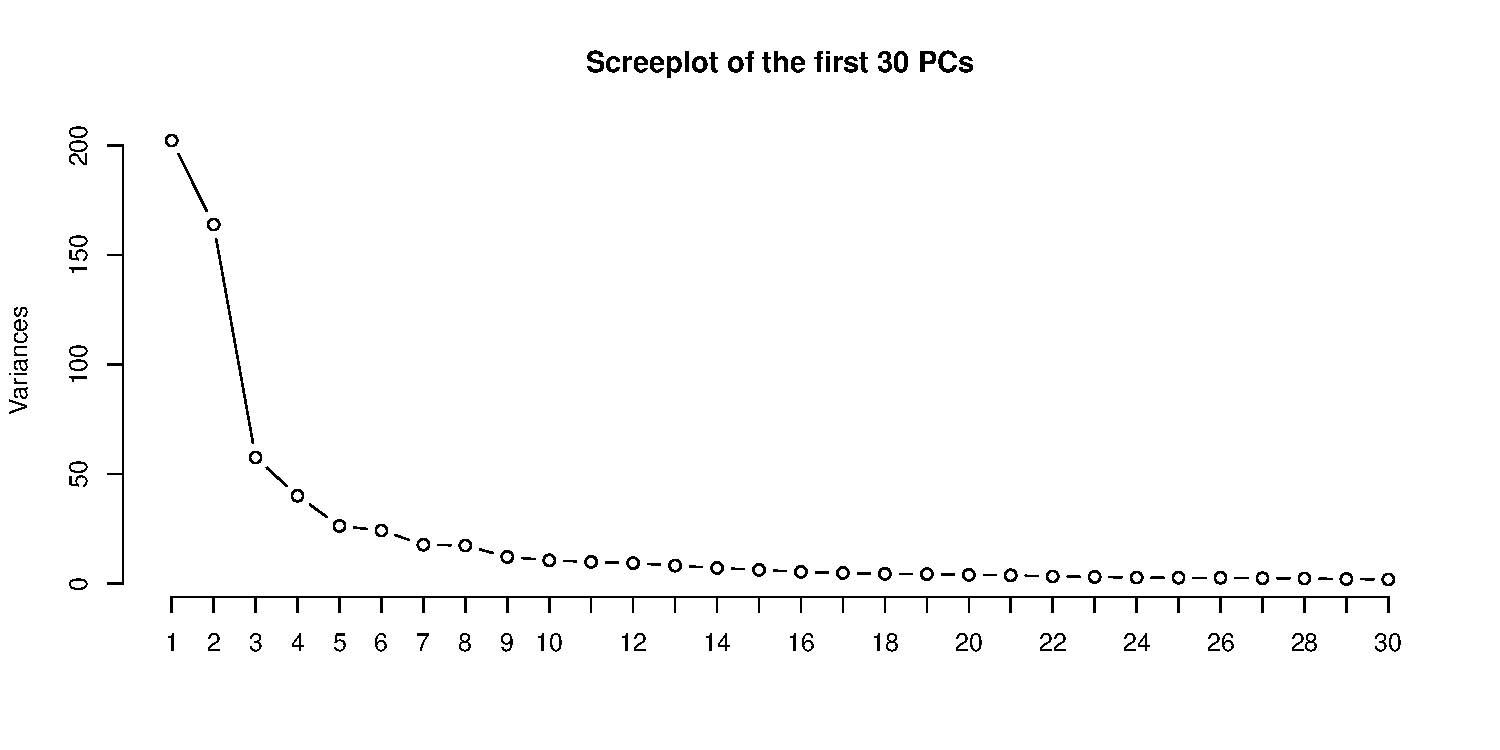
\includegraphics[width=1\linewidth]{Project2_as81_files/figure-latex/unnamed-chunk-17-1} \end{center}

\begin{center}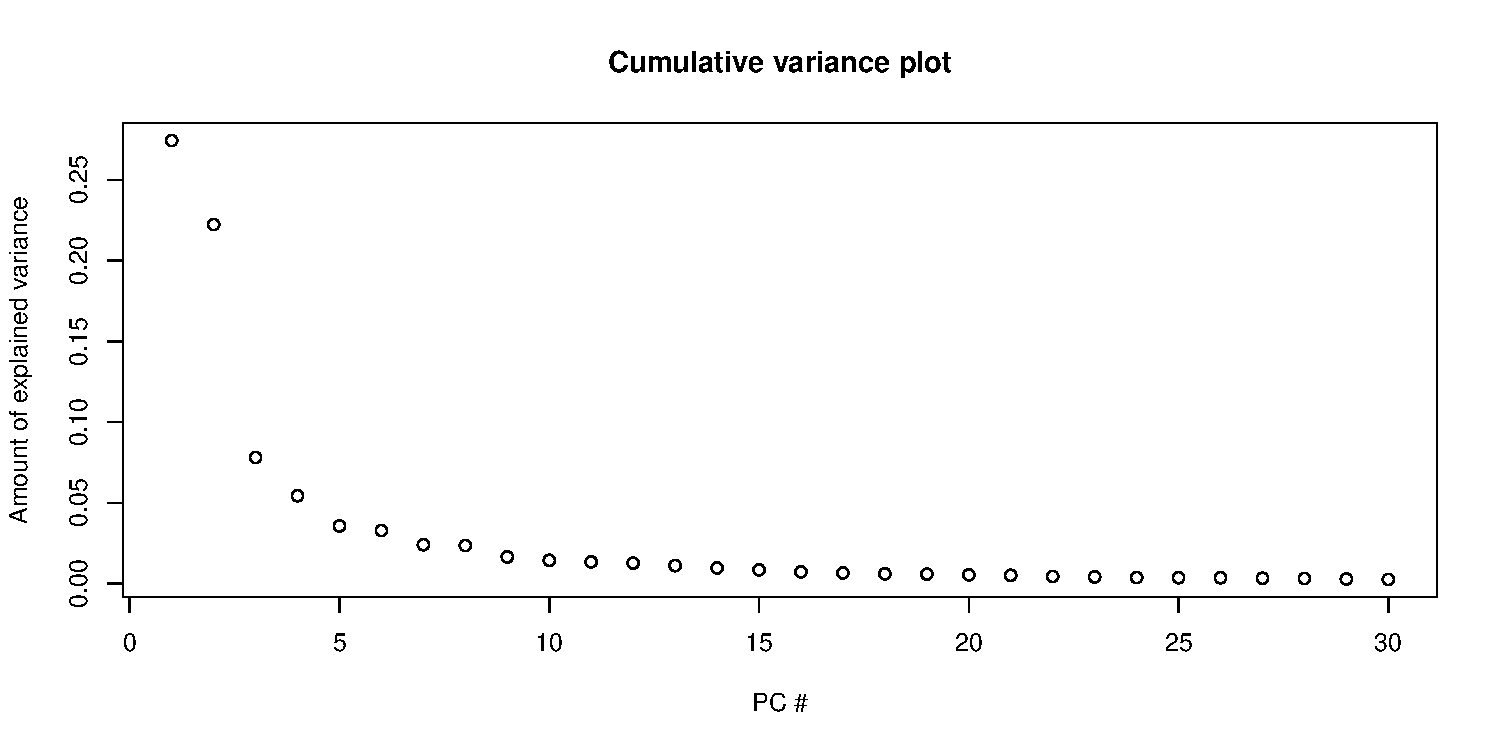
\includegraphics[width=1\linewidth]{Project2_as81_files/figure-latex/unnamed-chunk-18-1} \end{center}

\begin{center}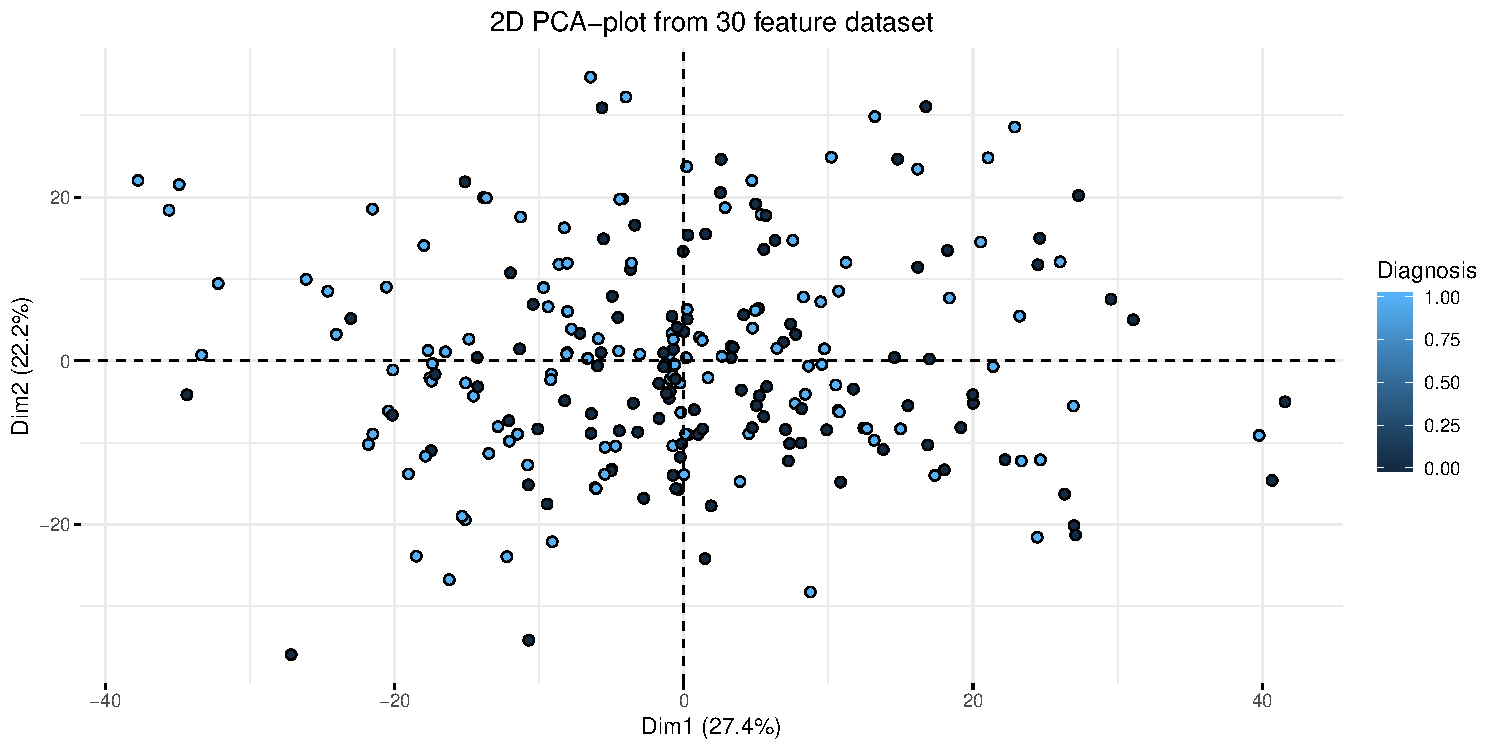
\includegraphics[width=1\linewidth]{Project2_as81_files/figure-latex/unnamed-chunk-19-1} \end{center}

\hypertarget{points-1-page-literature-review.-you-should-search-and-read-existing-literature-and-summarize-clinically-relevant-characteristics-that-could-be-used-for-skin-cancer-image-diagnosis.-there-is-no-limitation-on-what-type-of-literature-you-could-use.-however-the-goal-should-be-motivating-your-feature-engineering-approaches-from-a-clinical-and-analytic-point-of-view.-please-give-appropriate-citations-to-the-literature-you-read.}{%
\subsubsection{{[}10 Points, 1 page{]} Literature review. You should
search and read existing literature and summarize clinically relevant
characteristics that could be used for skin cancer image diagnosis.
There is no limitation on what type of literature you could use.
However, the goal should be motivating your feature engineering
approaches from a clinical and analytic point of view. Please give
appropriate citations to the literature you
read.}\label{points-1-page-literature-review.-you-should-search-and-read-existing-literature-and-summarize-clinically-relevant-characteristics-that-could-be-used-for-skin-cancer-image-diagnosis.-there-is-no-limitation-on-what-type-of-literature-you-could-use.-however-the-goal-should-be-motivating-your-feature-engineering-approaches-from-a-clinical-and-analytic-point-of-view.-please-give-appropriate-citations-to-the-literature-you-read.}}

1 page description goes here

\hypertarget{points-1-page-feature-engineering.-motivated-by-what-you-have-read-or-your-understanding-process-the-data-in-a-reasonable-way-such-that-the-new-variables-are-more-intuitive-to-your-collaboratorclinicians.-you-need-to-describe-clearly-what-is-your-data-processing-criteria-and-how-your-variables-are-calculated.}{%
\subsubsection{{[}10 Points, 1 page{]} Feature engineering. Motivated by
what you have read (or your understanding), process the data in a
reasonable way such that the new variables are more intuitive to your
collaborator/clinicians. You need to describe clearly what is your data
processing criteria and how your variables are
calculated.}\label{points-1-page-feature-engineering.-motivated-by-what-you-have-read-or-your-understanding-process-the-data-in-a-reasonable-way-such-that-the-new-variables-are-more-intuitive-to-your-collaboratorclinicians.-you-need-to-describe-clearly-what-is-your-data-processing-criteria-and-how-your-variables-are-calculated.}}

1 page description goes here

\hypertarget{points-2-page-classification-models-based-on-new-features.-fit-two-different-classification-models-to-identify-malignant-moles.-you-can-either-use-the-ones-from-question-1-or-use-some-new-models-if-you-believe-they-may-perform-better-on-the-new-features.-same-requirements-of-question-1-apply-to-this-part.-besides-you-should-focus-more-on-variable-selection-and-interpretation.}{%
\subsubsection{{[}20 Points, 2 page{]} Classification models based on
new features. Fit two different classification models to identify
malignant moles. You can either use the ones from Question 1 or use some
new models if you believe they may perform better on the new features.
Same requirements of Question 1 apply to this part. Besides, you should
focus more on variable selection and
interpretation.}\label{points-2-page-classification-models-based-on-new-features.-fit-two-different-classification-models-to-identify-malignant-moles.-you-can-either-use-the-ones-from-question-1-or-use-some-new-models-if-you-believe-they-may-perform-better-on-the-new-features.-same-requirements-of-question-1-apply-to-this-part.-besides-you-should-focus-more-on-variable-selection-and-interpretation.}}

\begin{Shaded}
\begin{Highlighting}[]
\CommentTok{# use parallel for performace }
  \KeywordTok{registerDoMC}\NormalTok{(}\DataTypeTok{cores =} \DecValTok{4}\NormalTok{)}

  \CommentTok{# Ridge Regression}
\NormalTok{  cv_glmnet_model <-}\StringTok{ }\KeywordTok{cv.glmnet}\NormalTok{(train.data[, }\DecValTok{-1}\NormalTok{], train.data[, }\DecValTok{1}\NormalTok{], }\DataTypeTok{parallel =} \OtherTok{TRUE}\NormalTok{, }\DataTypeTok{alpha=}\DecValTok{0}\NormalTok{, }\DataTypeTok{family=}\StringTok{"binomial"}\NormalTok{)}
\end{Highlighting}
\end{Shaded}

\begin{center}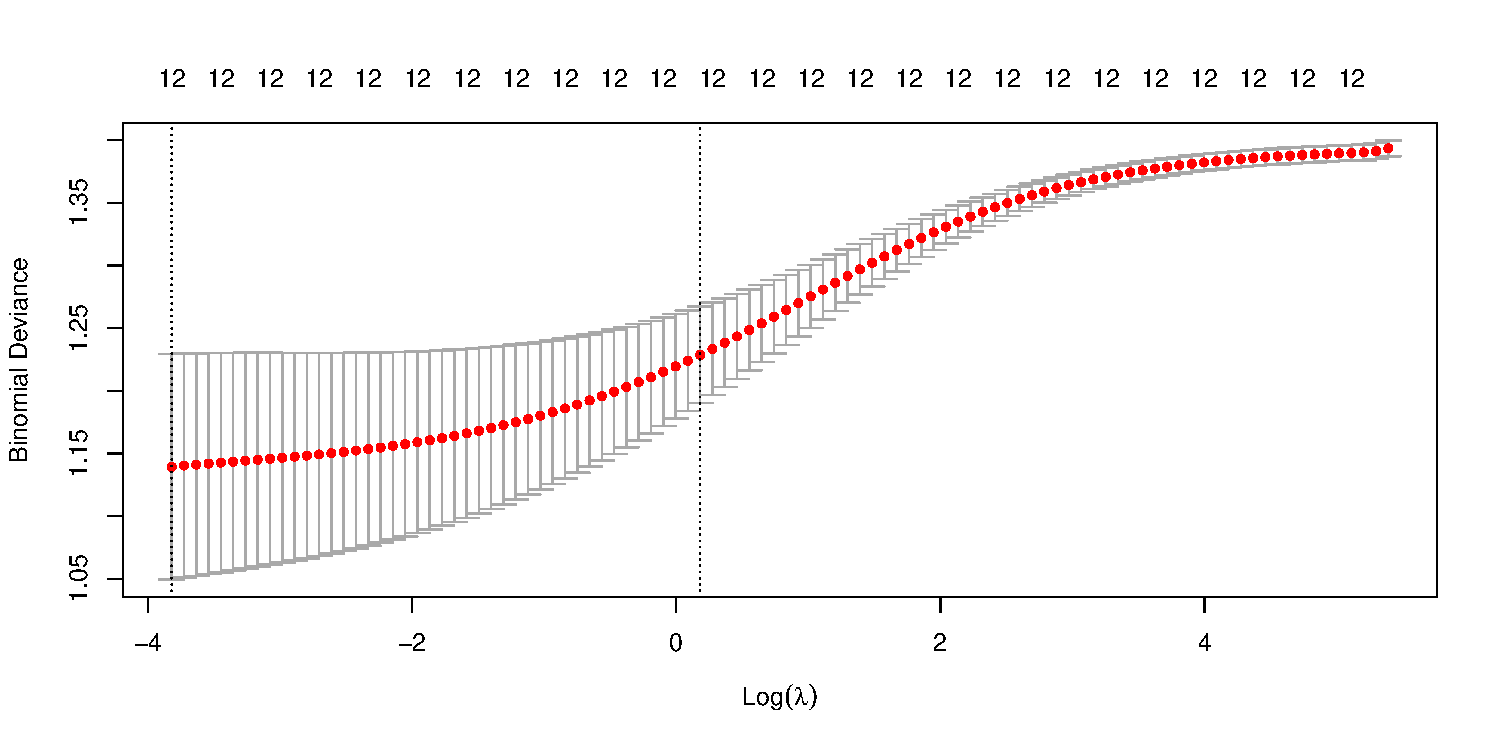
\includegraphics[width=1\linewidth]{Project2_as81_files/figure-latex/unnamed-chunk-35-1} \end{center}

\begin{Shaded}
\begin{Highlighting}[]
\NormalTok{  best_lambda =}\StringTok{ }\NormalTok{cv_glmnet_model}\OperatorTok{$}\NormalTok{lambda}\FloatTok{.1}\NormalTok{se}
  \CommentTok{# training with best lambda selected from the cv}
\NormalTok{  train_glmnet_model <-}\StringTok{ }\KeywordTok{glmnet}\NormalTok{(train.data[, }\DecValTok{-1}\NormalTok{], train.data[, }\DecValTok{1}\NormalTok{], }\DataTypeTok{lambda =}\NormalTok{ best_lambda, }\DataTypeTok{alpha=}\DecValTok{0}\NormalTok{, }\DataTypeTok{family=}\StringTok{"binomial"}\NormalTok{)}
  
  \KeywordTok{summary}\NormalTok{(train_glmnet_model)}
\end{Highlighting}
\end{Shaded}

\begin{verbatim}
##            Length Class     Mode     
## a0          1     -none-    numeric  
## beta       12     dgCMatrix S4       
## df          1     -none-    numeric  
## dim         2     -none-    numeric  
## lambda      1     -none-    numeric  
## dev.ratio   1     -none-    numeric  
## nulldev     1     -none-    numeric  
## npasses     1     -none-    numeric  
## jerr        1     -none-    numeric  
## offset      1     -none-    logical  
## classnames  2     -none-    character
## call        6     -none-    call     
## nobs        1     -none-    numeric
\end{verbatim}

\begin{Shaded}
\begin{Highlighting}[]
\NormalTok{  pred <-}\StringTok{ }\KeywordTok{predict}\NormalTok{(train_glmnet_model, }\DataTypeTok{s =}\NormalTok{ best_lambda, }\DataTypeTok{newx =}\NormalTok{ test.data[, }\DecValTok{-1}\NormalTok{], }\DataTypeTok{type =} \StringTok{"class"}\NormalTok{)}
\NormalTok{  accuracy =}\StringTok{ }\KeywordTok{mean}\NormalTok{(test.data[, }\DecValTok{1}\NormalTok{] }\OperatorTok{==}\StringTok{ }\NormalTok{pred)}
  
\NormalTok{  results =}\StringTok{ }\KeywordTok{data.frame}\NormalTok{(}\StringTok{"Best lambda"}\NormalTok{ =}\StringTok{ }\NormalTok{best_lambda, }\StringTok{"Accuracy"}\NormalTok{ =}\StringTok{ }\NormalTok{accuracy)}
\end{Highlighting}
\end{Shaded}

\begin{Shaded}
\begin{Highlighting}[]
  \KeywordTok{kable}\NormalTok{(results, }\DataTypeTok{caption =} \StringTok{"Ridge Regression Results"}\NormalTok{)}
\end{Highlighting}
\end{Shaded}

\begin{table}

\caption{\label{tab:unnamed-chunk-37}Ridge Regression Results}
\centering
\begin{tabular}[t]{r|r}
\hline
Best.lambda & Accuracy\\
\hline
1.198349 & 0.7\\
\hline
\end{tabular}
\end{table}

\end{document}
